\documentclass{beamer}
\mode<presentation>
\usepackage{color}
\usepackage{graphicx} % Required for inserting images
\usetheme{Berlin}

\definecolor{background}{RGB}{255,255,255}
\definecolor{textcolor}{RGB}{0,0,0}
\definecolor{ozadje}{RGB}{51,102,0}
\setbeamercolor{structure}{fg=ozadje}

\title{Napredna računalniška orodja}
\subtitle{Domača naloga 1}
\titlegraphic{
\includegraphics[scale=0.1]{UL-Fakulteta-za-strojnistvo.jpg}}
\author{Luka Uranič}
\institute{UL, Fakulteta za strojništvo}
\date{October 2023}

\begin{document}

\maketitle

\begin{frame}
\frametitle{KAZALO}
\tableofcontents
\end{frame}

\section{UVOD}
\begin{frame}
To je predstavitev, ki predstavlja potek prve domače naloge pri predmetu Napredna računalniška orodja, v kateri smo z uporabo generatorja naključnih števil, v programu Matlab, izračunali približek števila $\pi$ s pomočjo metode Monte carlo.
\begin{figure}[h!]
    \centering
    
\includegraphics[scale=0.12]{Matlab_LOGO.png}
    \caption{Logo Matlab}
    \label{fig:enter-label}
\end{figure}
\end{frame}

\section{IZRAČUN}
\begin{frame}
Izračun približka smo opravili v več korakih:
\begin{itemize}
  \pause
  \item<1-> Najprej smo definirali funkcijo \textbf{\texttt{mcc\_pi.m}}, ki nam naključne točke razporedi znotraj kvadrata in določi katere točke so znotraj kvadratu včrtanega kroga in katere zunaj kroga.
  \pause
  \item<2-> Ustvarili smo programsko datoteko z imenom \textbf{\texttt{calculate\_pi.m}}, ki izračuna približek vrednosti števila $\pi$ in napako s katero približek odstopa od prave vrednosti števila
\end{itemize}
\end{frame}

\section{REZULTAT}
\begin{frame}
    Kot rezultat nam funkcija vrne približek števila $\pi$ in graf na katerem so prikazane točke uporabljene v izračunu.

    \begin{figure}[h!]
        \centering
        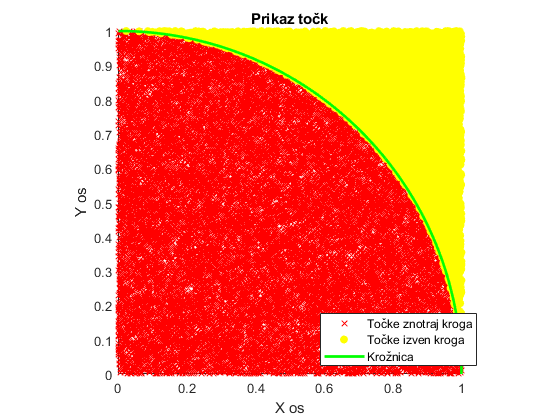
\includegraphics[scale=0.55]{graf_pi.png}
    \end{figure}
\end{frame}

\section{ZAKLJUČEK}
\begin{frame}
Z metodo Monte carlo smo lahko izračunali precej točno vrednost števila $\pi$, katere točnost je odvisna od števila naključno izbranih točk v kvadratu.
\end{frame}

\end{document}
